\section{Pronosticar la deriva de objetos en el océano}

El movimiento de un objeto a la deriva en la superficie del mar es uno 
de los temas de discusión fundamentales de este proyecto. Este
 movimiento es el resultado de varias fuerzas que actúan sobre la superficie:

\begin{enumerate}
\item Corrientes marinas.
\item Viento.
\item Oleaje.
\end{enumerate}


También influye el centro de gravedad del objeto y su forma.

Tenemos dos cuestiones importantes que definir, la dirección 
y la velocidad del objeto a la deriva.

\subsection{Velocidad del objeto}

Después de leer varios estudios y artículos, he llegado a la
 conclusión, que la fórmula para calcular la velocidad de un objeto 
flotando a la deriva, es directamente proporcional a la velocidad
del viento y condicionado por un factor que se calcula empíricamente
 o con modelos muy complejos de mecánica de fluidos que no 
tenemos a nuestra disposición, así que vamos a simplificar.

Utilizaremos la siguiente fórmula.
\[\
   x \times \alpha + A \\  
\]

Donde:
\begin{enumerate}
\item $x$ es la velocidad del viento, en m/s.
\item $alpha$ es el coeficiente con valor 0.70.
\item $A$ es la constante de error, que calculamos como un 20\% del valor de $x$.
\end{enumerate}

Fuente: Formulation of Leeway-Drift Velocities for Sea-Surface
Drifting-Objects Based on a Wind-Wave Flume Experiment~\cite{VDERIVA}.



\subsection{Dirección del objeto}


Otro de los puntos más importantes es la dirección de movimiento del 
objeto a la deriva, comúnmente se piensa que es la misma que la del viento,
 pero hay que tener en cuenta la componente cruzada del viento principal, a
 la hora de calcular esta dirección, podemos ver en la siguiente imagen como 
se compone el vector de movimiento del objeto a la deriva.


\begin{figure}[h]
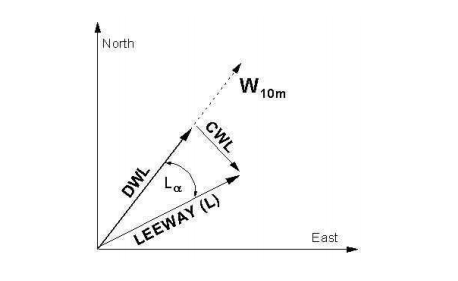
\includegraphics[scale=0.5]{relacion_viento.png} 
\caption{Relacion entre el vector del objeto a la deriva (L), 
el vector del viento (DWL) y el vector del viento cruzado (CWL). L indica el ángulo de deriva. }
\end{figure}


Para solventar en nuestro algoritmo el problema del viento cruzado, vamos a añadir un margen de 
error del treinta por ciento a la hora de calcular la dirección de deriva. 

Fuente: Ocean weather forecasting: An integrated view of oceanography~\cite{DDERIVA}.